\documentclass{beamer}

\mode<presentation> {

% The Beamer class comes with a number of default slide themes
% which change the colors and layouts of slides. Below this is a list
% of all the themes, uncomment each in turn to see what they look like.

%\usetheme{default}
%\usetheme{AnnArbor}
%\usetheme{Antibes}
%\usetheme{Bergen}
%\usetheme{Berkeley}
%\usetheme{Berlin}
%\usetheme{Boadilla}
%\usetheme{CambridgeUS}
%\usetheme{Copenhagen}
%\usetheme{Darmstadt}
%\usetheme{Dresden}
%\usetheme{Frankfurt}
%\usetheme{Goettingen}
%\usetheme{Hannover}
%\usetheme{Ilmenau}
%\usetheme{JuanLesPins}
%\usetheme{Luebeck}
\usetheme{Madrid}
%\usetheme{Malmoe}
%\usetheme{Marburg}
%\usetheme{Montpellier}
%\usetheme{PaloAlto}
%\usetheme{Pittsburgh}
%\usetheme{Rochester}
%\usetheme{Singapore}
%\usetheme{Szeged}
%\usetheme{Warsaw}

% As well as themes, the Beamer class has a number of color themes
% for any slide theme. Uncomment each of these in turn to see how it
% changes the colors of your current slide theme.

%\usecolortheme{albatross}
%\usecolortheme{beaver}
%\usecolortheme{beetle}
%\usecolortheme{crane}
%\usecolortheme{dolphin}
%\usecolortheme{dove}
%\usecolortheme{fly}
%\usecolortheme{lily}
%\usecolortheme{orchid}
%\usecolortheme{rose}
%\usecolortheme{seagull}
%\usecolortheme{seahorse}
%\usecolortheme{whale}
%\usecolortheme{wolverine}

%\setbeamertemplate{footline} % To remove the footer line in all slides uncomment this line
%\setbeamertemplate{footline}[page number] % To replace the footer line in all slides with a simple slide count uncomment this line

%\setbeamertemplate{navigation symbols}{} % To remove the navigation symbols from the bottom of all slides uncomment this line
}

\usepackage{graphicx} % Allows including images
\usepackage{booktabs} % Allows the use of \toprule, \midrule and \bottomrule in tables
\usepackage{amsmath}
\usepackage{xspace}
\usepackage{amssymb,amsmath,amsthm}
\usepackage{color}
\usepackage{epsfig}
\usepackage{algorithm2e}
\usepackage{algorithmic}
\usepackage{tabularx}
\usepackage{caption}
\usepackage{multirow}
\usepackage{bbm}
\usepackage[T1]{fontenc}
\usepackage{listings}
\definecolor{dkgreen}{rgb}{0,0.6,0}
\lstset{ %
  language=R,                     % the language of the code
  basicstyle=\ttfamily\tiny,       % the size of the fonts that are used for the code
  numbers=left,                   % where to put the line-numbers
  numberstyle=\tiny\color{gray},  % the style that is used for the line-numbers
  stepnumber=1,                   % the step between two line-numbers. If it's 1, each line
                                  % will be numbered
  numbersep=5pt,                  % how far the line-numbers are from the code
  backgroundcolor=\color{white},  % choose the background color. You must add \usepackage{color}
  showspaces=false,               % show spaces adding particular underscores
  showstringspaces=false,         % underline spaces within strings
  showtabs=false,                 % show tabs within strings adding particular underscores
  frame=single,                   % adds a frame around the code
  rulecolor=\color{black},        % if not set, the frame-color may be changed on line-breaks within not-black text (e.g. commens (green here))
  tabsize=2,                      % sets default tabsize to 2 spaces
  breaklines=true,                % sets automatic line breaking
  breakatwhitespace=false,        % sets if automatic breaks should only happen at whitespace
  title=\lstname,                 % show the filename of files included with \lstinputlisting;
                                  % also try caption instead of title
  keywordstyle=\color{blue},      % keyword style
  commentstyle=\color{green},   % comment style
  stringstyle=\color{mauve},      % string literal style
  escapeinside={\%*}{*)},         % if you want to add a comment within your code
  morekeywords={*,\ldots}            % if you want to add more keywords to the set
}
\definecolor{mauve}{rgb}{0.88, 0.69, 1.0}
%----------------------------------------------------------------------------------------
%	TITLE PAGE
%----------------------------------------------------------------------------------------

\title[Sparse Clustering]{A Framework for Feature Selection in Clustering} % The short title appears at the bottom of every slide, the full title is only on the title page

\author{Daniela M. Witten and Robert Tibshirani} % Your name
\institute[] % Your institution as it will appear on the bottom of every slide, may be shorthand to save space
{
Stanford University \\ % Your institution for the title page
\medskip
\textit{} % Your email address
}
\date{Wentao Wu} % Date, can be changed to a custom date

\begin{document}

\begin{frame}
\titlepage % Print the title page as the first slide
\end{frame}

\begin{frame}
\frametitle{Overview} % Table of contents slide, comment this block out to remove it
\tableofcontents % Throughout your presentation, if you choose to use \section{} and \subsection{} commands, these will automatically be printed on this slide as an overview of your presentation
\end{frame}

%----------------------------------------------------------------------------------------
%	PRESENTATION SLIDES
%----------------------------------------------------------------------------------------

%------------------------------------------------
\section{Problem} % Sections can be created in order to organize your presentation into discrete blocks, all sections and subsections are automatically printed in the table of contents as an overview of the talk
%------------------------------------------------

\begin{frame}
\frametitle{Problem}

\begin{itemize}
    \item Clustering: Given $X_{n\times p}$, identify $K$ clusters.
    \item Sparse Clustering: Underlying clusters only differ on $q < p$ features.
          \begin{itemize}
            \item improve accuracy and interpretation
            \item cheaper prediction
          \end{itemize}
\end{itemize}

\begin{figure}[h!]
  \centering
    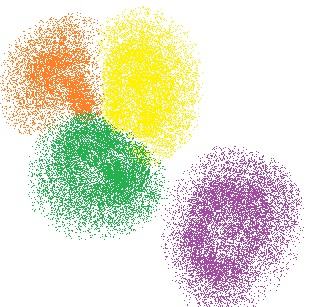
\includegraphics[width=0.4\textwidth]{cluster.jpeg}
\end{figure}


\end{frame}

%------------------------------------------------

\begin{frame}[fragile]
\frametitle{Motivating Example}
\begin{columns}[c] % The "c" option specifies centered vertical alignment while the "t" option is used for top vertical alignment

\column{.45\textwidth} % Left column and width
\begin{figure}[h!]
  \centering
    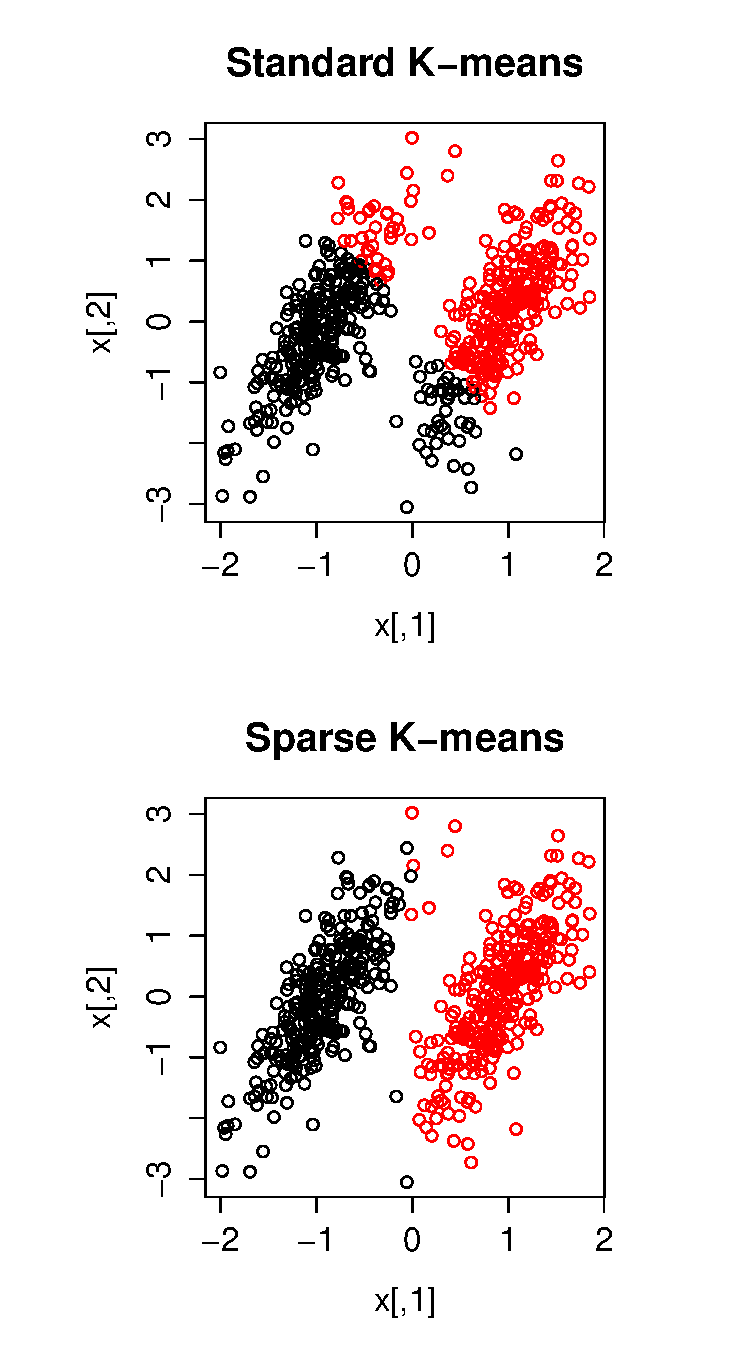
\includegraphics[width=0.7\textwidth]{example.pdf}
\end{figure}

\column{.5\textwidth} % Right column and width


\begin{equation*}
X_1 \sim N
\begin{bmatrix}
\begin{pmatrix}
-0.5\\
0
\end{pmatrix}\!\!,&
\begin{pmatrix}
1 & 0.78 \\
0.78 & 1
\end{pmatrix}
\end{bmatrix}
\end{equation*}
\begin{equation*}
X_2 \sim N
\begin{bmatrix}
\begin{pmatrix}
0.5\\
0
\end{pmatrix}\!\!,&
\begin{pmatrix}
1 & 0.78 \\
0.78 & 1
\end{pmatrix}
\end{bmatrix}
\end{equation*}

\begin{lstlisting}[language=R]
#K-means
cl <- kmeans(x,2)
plot(x,col=cl$cluster, main='Standard K-means')
#Sparse K-means
km.perm <- KMeansSparseCluster.permute(x,K=2,wbounds=seq(3,7,len=15),nperms=5)
km.out <- KMeansSparseCluster(x,K=2,wbounds=km.perm$bestw)
plot(x,col=km.out[[1]]$Cs, main='Sparse K-means')
\end{lstlisting}
\end{columns}
\end{frame}

%------------------------------------------------
\section{Proposed Framework}
\begin{frame}
\frametitle{Proposed Framework}
{\Large \bf Clustering}

\begin{equation*}
\max_{\Theta \in D}~~\sum_{j=1}^p f_j (X_j, \Theta)
\end{equation*}
\begin{itemize}
    \item $X_j \in \mathbbm{R}^n$ : feature $j$
    \item $\Theta$ : a parameter restricted to lie in set $D$.
    \item $f_j(X_j, \Theta)$ : some function that involves only the $j$th feature.
\end{itemize}
\end{frame}
%------------------------------------------------
\begin{frame}
\frametitle{Proposed Framework}
{\Large \bf Sparse Clustering}

\begin{eqnarray*}
\max_{\Theta \in D}&~~\sum_{j=1}^p w_jf_j (X_j, \Theta)\\
\text{subject to} &~~ \Vert w \Vert^2 \le 1,~\Vert w \Vert_1 \le s,~w_j \ge 0
\end{eqnarray*}
\begin{itemize}
    \item $w_j$ is a weight corresponding to feature $j$, also indicates contribution.
    \item $w_1=w_2=\ldots=w_p$, reduces to the traditional clustering.
    \item $L_1$ penalty results in sparsity.
    \item $L_2$ penalty avoids trivial solution, (at most one element of $w$ is nonzero).
\end{itemize}
\end{frame}
%------------------------------------------------
\begin{frame}
\frametitle{How to optimize}
\begin{itemize}
    \item Alternating Iterative Algorithm
    \item Holding $w$ fixed, optimize with respect to $\Theta$.
        \begin{itemize}
            \item Standard clustering procedure to a weighted version of the data.
        \end{itemize}
    \item Holding $\Theta$ fixed, optimize with respect to $w$.
        \begin{itemize}
            \item $w = \frac{S(a_{+}, \Delta)}{\Vert S(a_{+},\Delta) \Vert^2}$.
            \begin{itemize}
            \item $a = f_j(X_j, \Theta)$.
            \item $S(x,c) = \text{sign}(x)(\vert x \vert - c)_{+}$.
            \item $\Delta=0$ if that results in $\Vert w \Vert_1 \le s$, otherwise, $\Delta > 0$ is chosen to yield $\Vert w \Vert_1 = s$.
            \end{itemize}
        \end{itemize}
\end{itemize}
\end{frame}
%------------------------------------------------
\begin{frame}
\frametitle{How to optimize}

\begin{eqnarray*}
\max_{w} & w^Ta\\
\text{subject to } & \Vert w \Vert^2 \le 1,~ \Vert w \Vert_1 \le s, ~ w_j \ge 0
\end{eqnarray*}

Introducing Lagrangian multipliers $\lambda_1$ for $\Vert w \Vert^2 -1 \le 0$, $\lambda_2$ for $\Vert w \Vert_1 - s \le 0$ and $\mu_j$ for $w_j \ge 0$. We obtain the KKT condition:
\begin{eqnarray*}
 w^T w -1 \le 0 ~&~
 \sum w_j -s \le 0\\
 \mu_j w_j  \le 0 ~&~
 w_j  \ge 0\\
 \lambda_1 (w^T w -1 ) = 0 ~&~
 \lambda_2 (\sum w_j -s ) = 0\\
 \mu_j w_j =0 ~&~
 -a + \lambda_1 w_j + \lambda_2 - \mu_j =0
\end{eqnarray*}
\end{frame}
%------------------------------------------------
\begin{frame}
\frametitle{How to optimize}
Based on the last equation, $\mu_j = -a + \lambda_1 w_j + \lambda_2$. Thus, $(-a + \lambda_2 + \lambda_1 w_j) w_j = 0$.
\begin{itemize}
 \item Case 1: $\sum w_j -s < 0$. Thus, $\lambda_2 = 0$. If $a < 0$, then $w_j = 0$. Otherwise, $w_j = \frac{a}{\lambda_1}$, where $ \lambda_1 $ make sure that $w^T w = 1$.
 \item Case 2: $\sum w_j -s = 0$. Thus, $\lambda_2 \ge 0$. If $a < 0$, then $w_j = 0$. Otherwise, $w_j = \frac{a - \lambda_2}{\lambda_1}$, where $\lambda_1$ ensures that $w^T w = 1$ and $\lambda_2$ ensures $\sum w_j -s = 0$.
\end{itemize}
In summary,
\begin{equation*}
w = \frac{S(a_{+}, \Delta)}{\Vert S(a_{+},\Delta) \Vert^2}
\end{equation*}
\end{frame}
%------------------------------------------------

\section{Sparse K-Means}
%------------------------------------------------
\begin{frame}
\frametitle{Sparse K-Means Clustering}
{\Large \bf Standard K-Means}

\begin{equation*}
\max_{C_1,C_2,\ldots,C_K} ~~ \sum_{k=1}^K \frac{1}{n_k} \sum_{i,i' \in C_k} \sum_{j=1}^p d_{i,i',j}
\end{equation*}

\begin{itemize}
    \item $K$ is the number of clusters.
    \item $n_k$ is the number of observations in cluster $k$.
    \item $C_k$ contains the indices of the observations in cluster $k$.
    \item $d_{i,i',j}$ is the dissimilarity measure between observation $i$ and $i'$ along feature $j$.
\end{itemize}

\end{frame}
%------------------------------------------------
\begin{frame}
\frametitle{Sparse K-Means Clustering}
{\Large \bf Sparse K-Means}

\begin{eqnarray*}
\max_{C_1,C_2,\ldots,C_K,w} ~&~ \sum_{j=1}^p w_j(\frac{1}{n} \sum_{i=1}^n \sum_{i'=1}^n d_{i,i',j} - \sum_{k=1}^K \frac{1}{n_k} \sum_{i,i' \in C_k} d_{i,i',j} ) \\
\text{subject to } ~&~ \Vert w \Vert^2 \le 1, \quad \Vert w \Vert_1 \le s, \quad w_j \ge 0
\end{eqnarray*}
\begin{itemize}
    \item $w$ is the weight for each feature.
    \item $K$ is the number of clusters.
    \item $n_k$ is the number of observations in cluster $k$.
    \item $C_k$ contains the indices of the observations in cluster $k$.
    \item $d_{i,i',j}$ is the dissimilarity measure between observation $i$ and $i'$ along feature $j$.
\end{itemize}
\end{frame}
%------------------------------------------------
\begin{frame}
\frametitle{Optimize Sparse K-Means Clustering}
\begin{enumerate}
\item Initialize $w$ as $w_i = \frac{1}{\sqrt{p}}$, where $i = 1, \ldots, p$.
\item Iterative until convergence $\frac{ \sum_{j=1}^p \vert w_j^r - w_j^{r-1} \vert}{\sum_j=1^p \vert w_j^{r-1} \vert} < 10^{-4}$.
    \begin{enumerate}
    \item Holding $w$ fixed, optimize with respect to $C_1, \ldots, C_K$. Applying the standard K-means algorithm to the $n \times n$ dissimilarity matrix with $(i,i')$ element $\sum_j w_j d_{i,i',j}$.
    \item Holding $C_1,\ldots, C_K$ fixed, optimize with respect to $w$ by applying
$$
w = \frac{S(a_+, \Delta)}{\Vert S(a_+,\Delta) \Vert^2}
$$
where
$
a_j = \frac{1}{n} \sum_{i=1}^n \sum_{i'=1}^n d_{i,i',j} - \sum_{k=1}^K \frac{1}{n_k} \sum_{i,i' \in C_k} d_{i,i',j}
$
    \end{enumerate}
\item The clusters are given by $C_1,\ldots, C_K$ and the feature weights corresponding to this clustering are given by $w_1, \ldots, w_p$.
\end{enumerate}
\end{frame}
%------------------------------------------------
\begin{frame}
\frametitle{Tuning Parameter}

\begin{itemize}
    \item $s$ the $L_1$ bound on $w$.
    \item Use gap statistics.
    \item Gap statistic measures the strength of the clustering obtained on the real data relative to the clustering obtained on null data that does not contain subgroups.
\end{itemize}

\end{frame}
%------------------------------------------------
\begin{frame}
\frametitle{Tuning Parameter}
\begin{enumerate}
\item Obtain permuted datasets $X_1,\ldots, X_B$ by independently permuting the observations within each feature.
\item For each candidate tuning parameter value $s$:
    \begin{enumerate}
    \item Compute
$
O(s) = \sum_j w_j (\frac{1}{n} \sum_{i=1}^n \sum_{i'=1}^n d_{i,i',j} - \sum_{k=1}^K \frac{1}{n_k} \sum_{i,i' \in C_k} d_{i,i',j} )
$
the objective obtained by performing sparse K-means with tuning parameter $s$ on the data $X$.
   \item For $b = 1,\ldots,B$, compute $O_b(s)$, the objective obtained by performing sparse K-means with tuning parameter value $s$ on the data $X_b$.
   \item Calculate $gap(s) = \text{log }(O(s)) - \frac{1}{B} \sum_{b=1}^B \text{log }(O_b(s))$.
   \end{enumerate}
\item Choose $s^*$ corresponding to the largest value of $gap(s)$.  Alternately, choose $s^*$ to equal the smallest value for which $gap(s^*)$ is within a standard deviation of $\text{log}(O_b(s^*))$ of the largest value of $gap(s)$.
\end{enumerate}
\end{frame}
%------------------------------------------------
\begin{frame}
\frametitle{Simulation}
\begin{itemize}
    \item Three Clusters: $C_1,C_2,C_3$.
    \item Each cluster contains $20$ observations.
    \item $p=100,q=50$: $100$ features, the underlying clusters depend on the first $50$ features.
    \item $X_{ij} \sim N(\mu_{ij},1)$.
    \item If $i \in C_k$ and $j \le q$, $\mu_{ij} = \mu_{c_k}$, where $\mu_{c_1}= 0,\mu_{c_2}=0.6,\mu_{c_3}=1.2$.
    \item If $j > q$, $\mu_{ij} = 0$ regardless of $i$.
    \item Metric: Rand index
\end{itemize}

\end{frame}

%------------------------------------------------
\begin{frame}
\frametitle{Simulation-Different $S$}

\begin{figure}[h!]
  \centering
    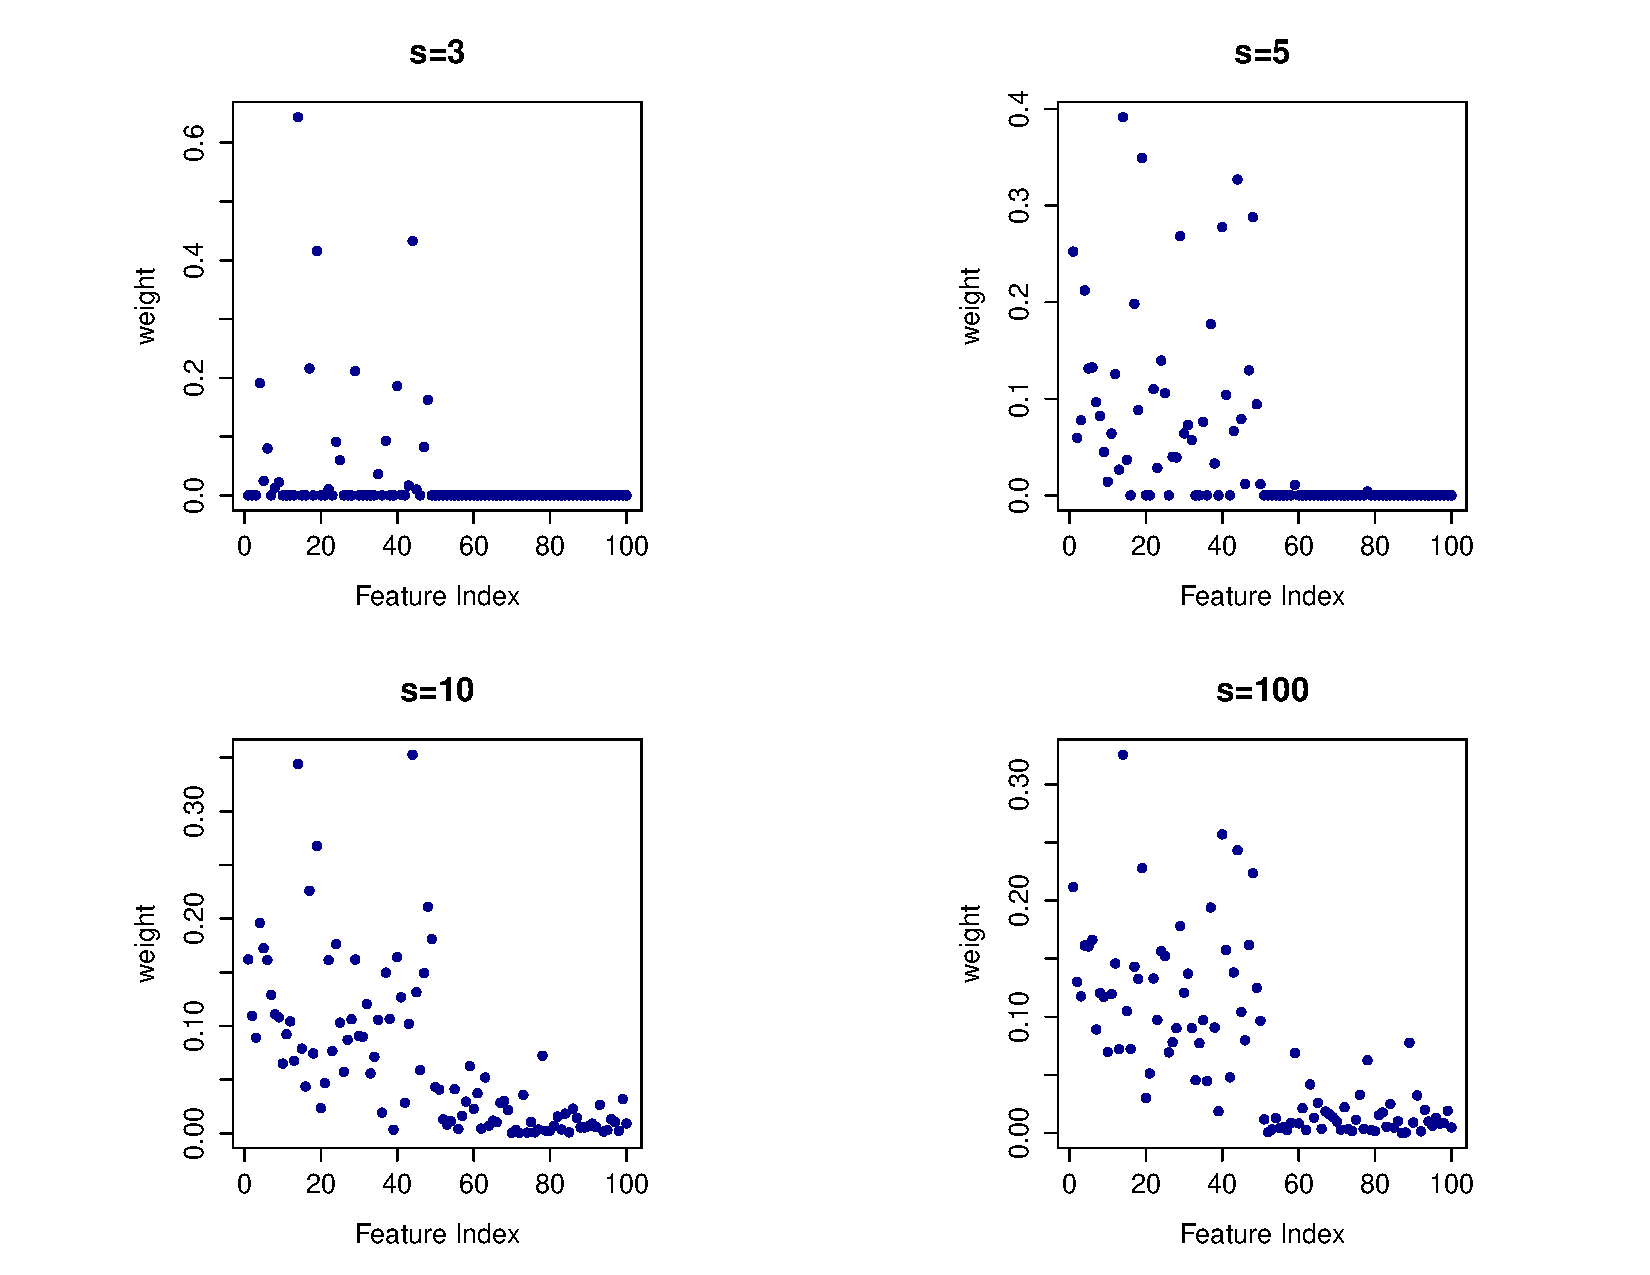
\includegraphics[width=0.9\textwidth]{varS.pdf}
\end{figure}
\end{frame}
%------------------------------------------------
\begin{frame}
\frametitle{Simulation-Different $p$}
\begin{figure}[h!]
  \centering
    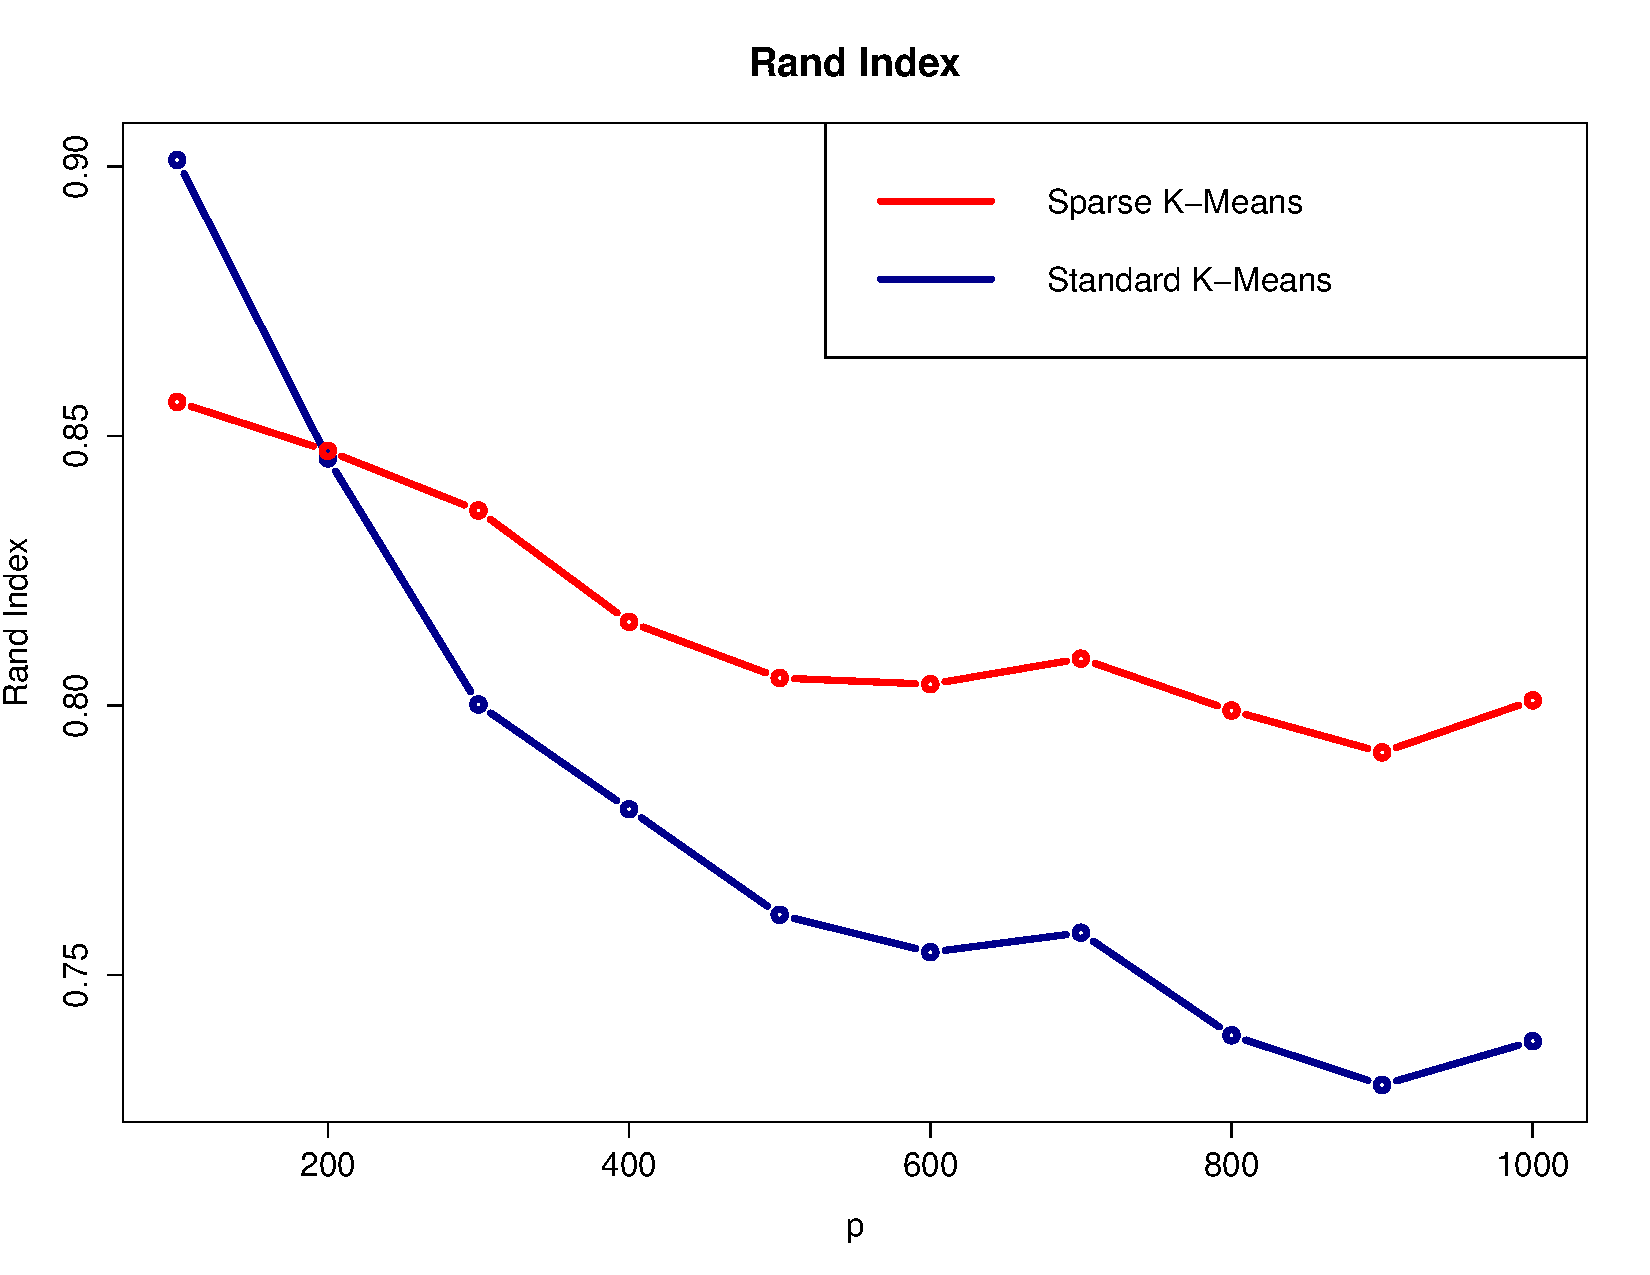
\includegraphics[width=0.8\textwidth]{randIndex.pdf}
\end{figure}
\end{frame}


%------------------------------------------------
\begin{frame}[fragile]
\frametitle{Simulation-Tuning}
\begin{lstlisting}
k.perm <- SparseKMeansTuning(x,K=3,wbounds=seq(3,10,len=15), nperm=10)
\end{lstlisting}

\begin{figure}[h!]
  \centering
    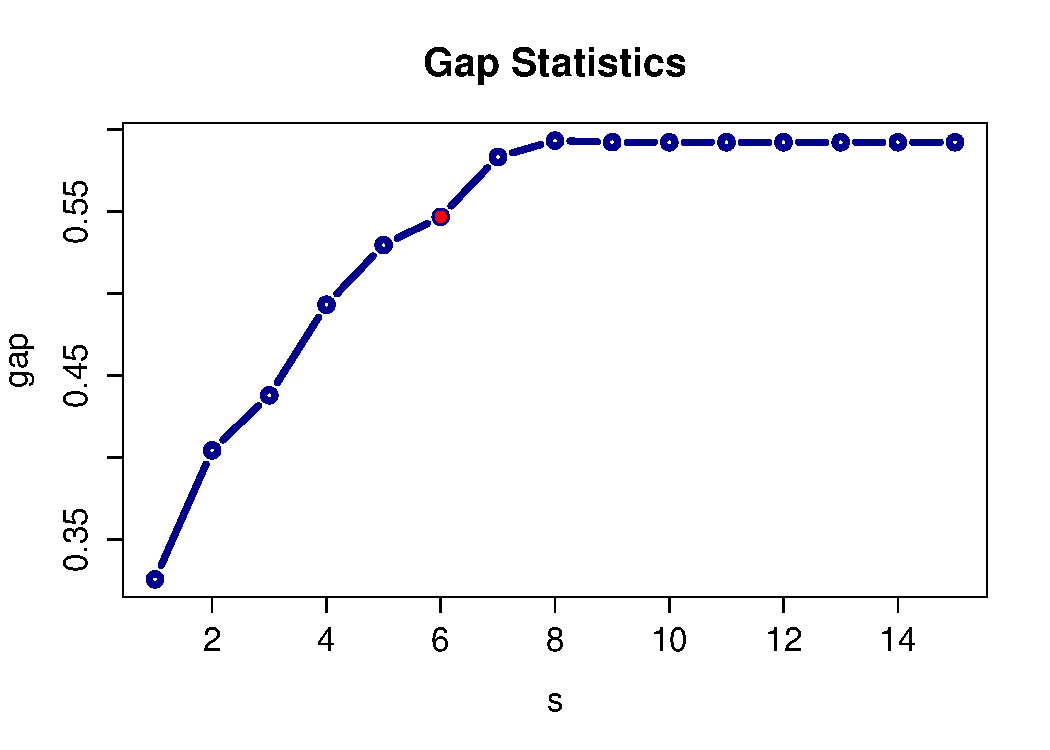
\includegraphics[width=0.7\textwidth]{gap.pdf}
\end{figure}
\end{frame}
%------------------------------------------------
\begin{frame}[fragile]
\frametitle{Simulation-Tuning}
\begin{lstlisting}
k.perm <- SparseKMeansTuning(x,K=3,wbounds=seq(3,10,len=15), nperm=10)
\end{lstlisting}

\begin{figure}[h!]
  \centering
    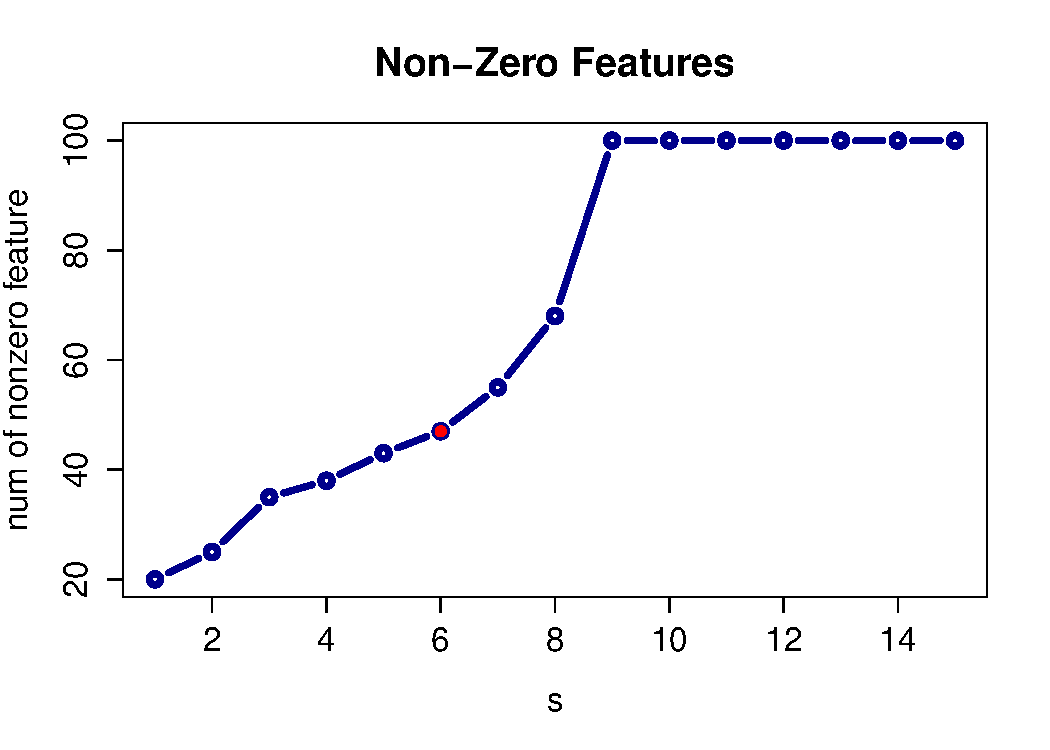
\includegraphics[width=0.7\textwidth]{nonzerofeature.pdf}
\end{figure}
\end{frame}


\section{Hierarchical Clustering}
%------------------------------------------------
\begin{frame}
\frametitle{Sparse Hierarchical Clustering}
{\Large \bf Standard Hierarchical}
\begin{eqnarray*}
\max_U &~ \{ \sum_j \sum_{i,i'} d_{i,i',j} U_{i,i'} \} \\
\text{subject to } & \sum_{i,i'} U^2_{i,i'} \le 1
\end{eqnarray*}

\begin{itemize}
    \item $U_{i,i'} \propto \sum_j d_{i,i'j}$.
    \item Performing hierarchical clustering on $U$ results in the standard hierarchical clustering.
\end{itemize}

\end{frame}
%------------------------------------------------
\begin{frame}
\frametitle{Sparse Hierarchical Clustering}
{\Large \bf Sparse Hierarchical}
\begin{eqnarray*}
\max_U &~ \{ \sum_j \sum_{i,i'} w_j d_{i,i',j} U_{i,i'} \} \\
\text{subject to } &~ \sum_{i,i'} U^2_{i,i'} \le 1,~ \Vert w \Vert^2 \le 1,~ \Vert w \Vert_1 \le s, ~ w_j \ge 0
\end{eqnarray*}
\begin{itemize}
    \item $U_{i,i'} \propto \sum_j w_j d_{i,i'j}$.
    \item Performing hierarchical clustering on $U$ results in the sparse hierarchical clustering.
\end{itemize}

\end{frame}
%------------------------------------------------
\begin{frame}
\frametitle{How to optimize}
\begin{enumerate}
\item Initialize $w$ as $w_1=\ldots=w_p=\frac{1}{\sqrt{p}}$.
\item Iterate until convergence:
    \begin{enumerate}
        \item  Update $u = \frac{Dw}{\Vert Dw \Vert_2}$.
        \item  Update $w = \frac{S(a_{+},\Delta)}{\Vert S(a_{+},\Delta) \Vert_2}$ where $a = D^Tu$ and $\Delta = 0$ if this results in $\Vert w \Vert_1 \le s$; otherwise, $\Delta > 0$ is chosen such that $\Vert w \Vert_1 = s$.
    \end{enumerate}
\item Rewrite $u$ as a $n \times n$ matrix $U$.
\item Perform hierarchical clustering on the $n \times n$ dissimilarity matrix $U$.
\end{enumerate}
\end{frame}
%------------------------------------------------


%------------------------------------------------

\begin{frame}
\Huge{\centerline{The End}}
\end{frame}

%----------------------------------------------------------------------------------------

\end{document}